


%\section{ニューラルネットワークを用いた自然言語処理}

本課題では,ニューラルネットワークを利用した自然言語処理の中核的な技術
である,sequence-to-sequence モデル(以下,seq2seqモデル)の基本的な原理と動作を学ぶ.
Seq2seq モデルは,単語列や文字列といった「系列」を入力し,新たな系列を出
力することのできるニューラルネットワークモデルであり,機械翻訳や質問応答,対話といっ
た様々な言語処理タスクへの応用が急速に進んでいる.なかでも機械翻訳に関しては,
近年の翻訳精度の向上に大きく貢献し,従来の統計的機械翻訳よりも格段に流暢な
翻訳を可能にしている \cite{wu2016google}.


%\subsection{単語ベクトル}
%
%Seq2seqモデルでは,単語を実数値のベクトルとして表現する.
%
%ニューラルネットワークを用いた自然言語処理では,単語を実数値のベクトルで表すことが多い.
%
%ベクトルの近さや cos類似度が単語の文法的・意味的な近さを表す.
%
%単語ベクトルの代表的な学習法を紹介する.
%
%
%\subsection{CBOWモデル}
%
%
%\subsection{Skip gram モデル}
%
%Skip gram モデル \cite{NIPS2013_5021} を説明する.

%\begin{equation}
%\frac{1}{T} \sum_{t=1}^T \sum_{-c \leq j \leq c, j \neq 0} \log p(w_{t+j} | w_t)
%\end{equation}
%
%$p(w_{t+j} | w_t)$ は以下のようにソフトマックス関数で定義される.
%%\begin{equation}
%p(w_O | w_I) = \frac{\exp({v'_{w_O}}^\top v_{w_I})}{ \sum_{w=1}^{W} \exp({v'_w}^\top v_{w_I})} 
%\end{equation}
%
%
%\subsection{実験課題}
%
%
%https://github.com/chainer/chainer/tree/master/examples/word2vec


\section{リカレントニューラルネットワーク}
\label{sec:rnn}

自然言語処理では,文字列や単語列といった「系列」を扱う処理が多い.しかし,通常のフィード
フォワードニューラルネットワークでは,入力と出力の次元数は固定されており,任意の
長さを持つ系列を扱う処理には適さない.
それに対して,
リカレントニューラルネットワーク (recurrent neural network, RNN) では,ネットワークに「状態」
を持たせることによって,任意の長さの系列を扱うことを可能にしている.


\begin{figure}[b]
 \begin{center}
  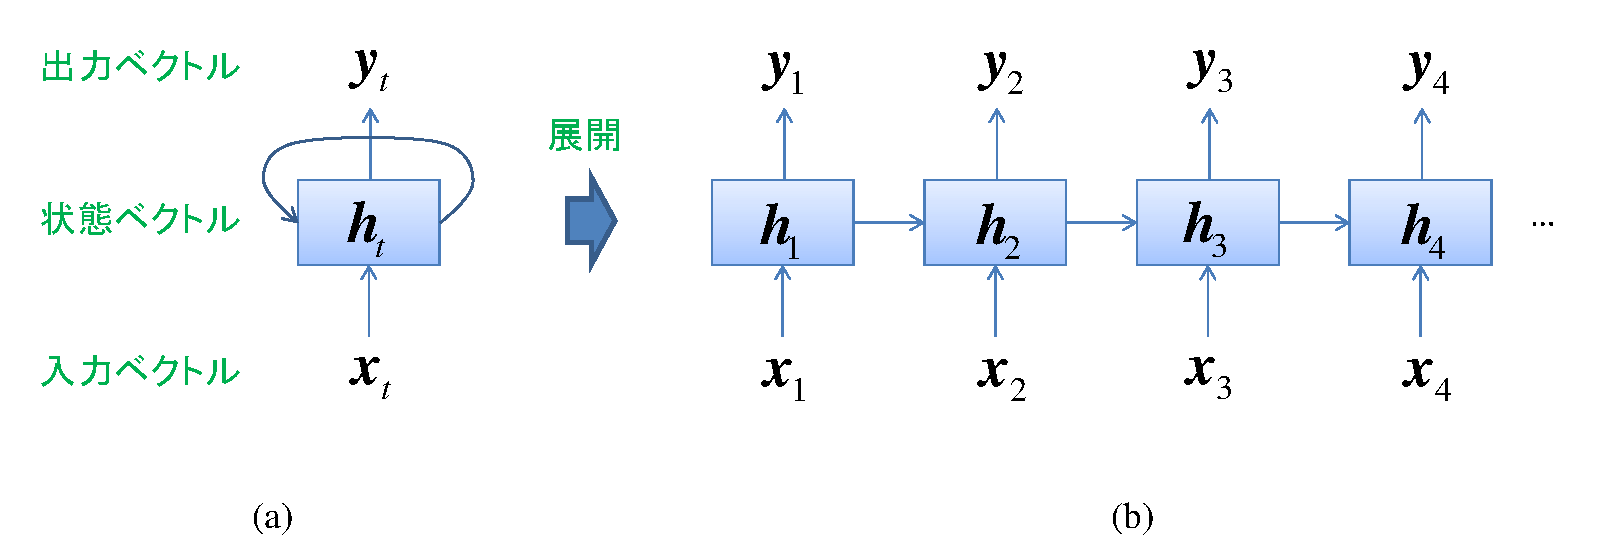
\includegraphics[width=140mm]{images/TsuruokaLab/rnn1.eps}
 \end{center}
 \caption{リカレントニューラルネットワーク}
 \label{fig:rnn1}
\end{figure}

図\ref{fig:rnn1}にリカレントニューラルネットワークの構造を示す.図\ref{fig:rnn1}(a)に示すように,
リカレントニューラルネットワークでは,ネットワーク自身が状態$\boldsymbol{h_t} \in \mathbb{R}^H$ を持つ
ことによって,その時点での入力$\boldsymbol{x}_t \in \mathbb{R}^D$ だけではなく,過去の入力
$\boldsymbol{x}_1,\boldsymbol{x}_2,...,\boldsymbol{x}_{t-1}$ にも
依存するような値$\boldsymbol{y_t} \in \mathbb{R}^V$ を出力することができる.
単純なリカレントニューラルネットワークでは,状態$\boldsymbol{h_t}$ は,
\begin{equation}
\boldsymbol{h_t} = \tanh(\boldsymbol{W}_h \boldsymbol{x}_{t} + \boldsymbol{U}_h \boldsymbol{h}_{t-1} + \boldsymbol{b}_h)
\end{equation}

\noindent
と計算される.ここで,$\boldsymbol{W}_h \in \mathbb{R}^{H \times D}$,$\boldsymbol{U}_h \in \mathbb{R}^{H \times H}$,
$\boldsymbol{b}_h \in \mathbb{R}^D$ は,このリカレントニューラルネットワークの動作を決めるパラメータである.

リカレントニューラルネットワークは,一見普通のフィードフォワードニューラルネットワークと大きく異なる
仕組みのように見えるが,実は本質的には通常のフィードフォワードニューラルネットワークと同じものである.
図\ref{fig:rnn1}(a)のリカレントニューラルネットワークを時間方向に展開して考えると,
図\ref{fig:rnn1}(b)に示すように,
パラメータ $\boldsymbol{W}_h$,$\boldsymbol{U}_h$,$\boldsymbol{b}_h$ を共有した多数のフィードフォワードネットワーク
を連結したものと等価であることがわかる.したがって,パラメータの学習も通常のフィードフォワードニューラルネットワーク同様,
誤差逆伝播法 (backpropagation) によって効率的に行うことができる.


\section{言語モデル}

\begin{figure}[t]
 \begin{center}
  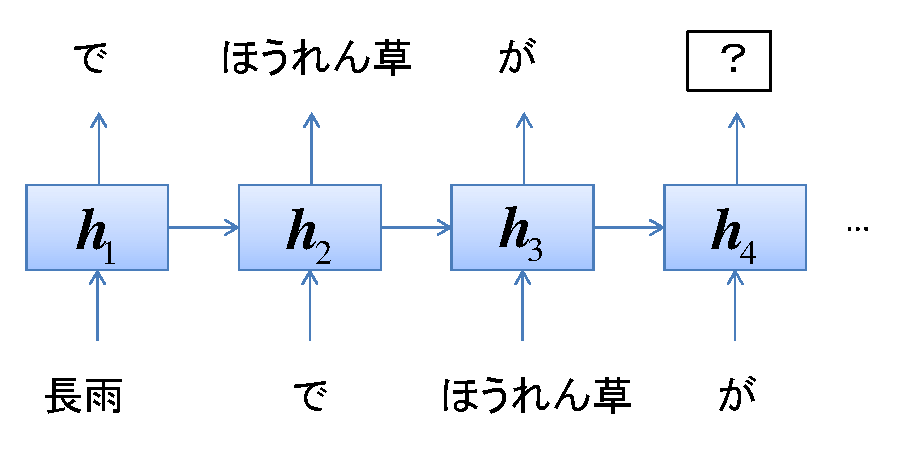
\includegraphics[width=80mm]{images/TsuruokaLab/lm.eps}
 \end{center}
 \caption{言語モデル}
 \label{fig:lm}
\end{figure}

リカレントニューラルネットワークを利用すると言語モデル(language model)を容易に実現することができる \cite{mikolov10lm}.
言語モデルでは,単語列$w_1,w_2,...,w_n$の生成を以下のような確率モデルで表現する.
\begin{equation}
P(w_1,w_2,...,w_n) = \prod_{t=1}^n P(w_t | w_1,...,w_{t-1})
\end{equation}

ここで図\ref{fig:lm}のように,リカレントニューラルネットワークの入力として,単語列$w_1,w_2,...,w_{t-1}$ 
% に対応するベクトルの列$\boldsymbol{x}_1,\boldsymbol{x}_2,...,\boldsymbol{x}_{t-1}$
を考え,出力として,単語列$w_2,w_3,...,w_{t}$
を考えれば,文脈$w_1,...,w_{t-1}$ から,次に出現するであろう単語$w_t$ を予測する
モデル $P(w_t | w_1,...,w_{t-1})$ が実現できることになる.$P(w_t | w_1,...,w_{t-1})$ は,可能性のある
すべての単語に関して和をとると 1 になる,すなわち単語の語彙に関する確率分布となっている必要あるため,
出力$\boldsymbol{y}_t$ は,ソフトマックス関数
\begin{equation}
\mbox{softmax}(\boldsymbol{a}): 
 \begin{bmatrix}
   a_1 \\
   a_2 \\
    : \\
   a_V \\
 \end{bmatrix}
~~\rightarrow~~
\frac{1}{\sum_{i=1}^V \exp(a_i)}
 \begin{bmatrix}
   \exp(a_1) \\
   \exp(a_2) \\
    : \\
   \exp(a_V) \\
\end{bmatrix}
\end{equation}
\noindent
を用いて
\begin{equation}
\boldsymbol{y_t} = \mbox{softmax}(\boldsymbol{U}_y \boldsymbol{h}_{t} + \boldsymbol{b}_y)
\end{equation}

\noindent
と計算すればよい.ここで,$\boldsymbol{U}_y \in \mathbb{R}^{V \times H}$ と $\boldsymbol{b}_y \in \mathbb{R}^{V}$
は,このリカレントニューラルネットワークの出力動作を規定するパラメータである.

%#ソフトマックスの説明

%ロス関数は,モデルの対数尤度を最大化(クロスエントロピーを最小化)する.

パラメータの学習は,学習データ(コーパス)でのモデルの対数尤度
\begin{equation}
J(\boldsymbol{\theta}) = \frac{1}{N} \sum_{i=1}^{N} \log P_{\boldsymbol{\theta}}(w_i | w_1,...,w_{i-1})
\end{equation}

\noindent
を最大化するように行う.ただし,$N$ は学習コーパスの単語数,$\boldsymbol{\theta}$ は
リカレントニューラルネットワークのすべてのパラメータを表す.


%\begin{equation}
%P_{RNN}(w_i | h_i)  = \frac{\exp(\theta_i^T v_{i-1})}{\sum_{j=1}^{|V|} \exp(\theta_i^T v_{i-1})}
%\end{equation}


\section{Long Short-Term Memory}

実は,\ref{sec:rnn}節で説明したような単純なリカレントニューラルネットワークでは,
高性能な言語モデルや翻訳モデルを実現することは難しい.言語現象を高い精度で再現する
ためには,遠く離れた単語間の依存関係もとらえる必要があるが,単純な
リカレントニューラルネットワークでは,誤差逆伝播を行う際の「勾配消失」と呼ばれる問題によって,
長距離依存関係をうまく学習することができないことが知られている.

\begin{figure}[t]
 \begin{center}
  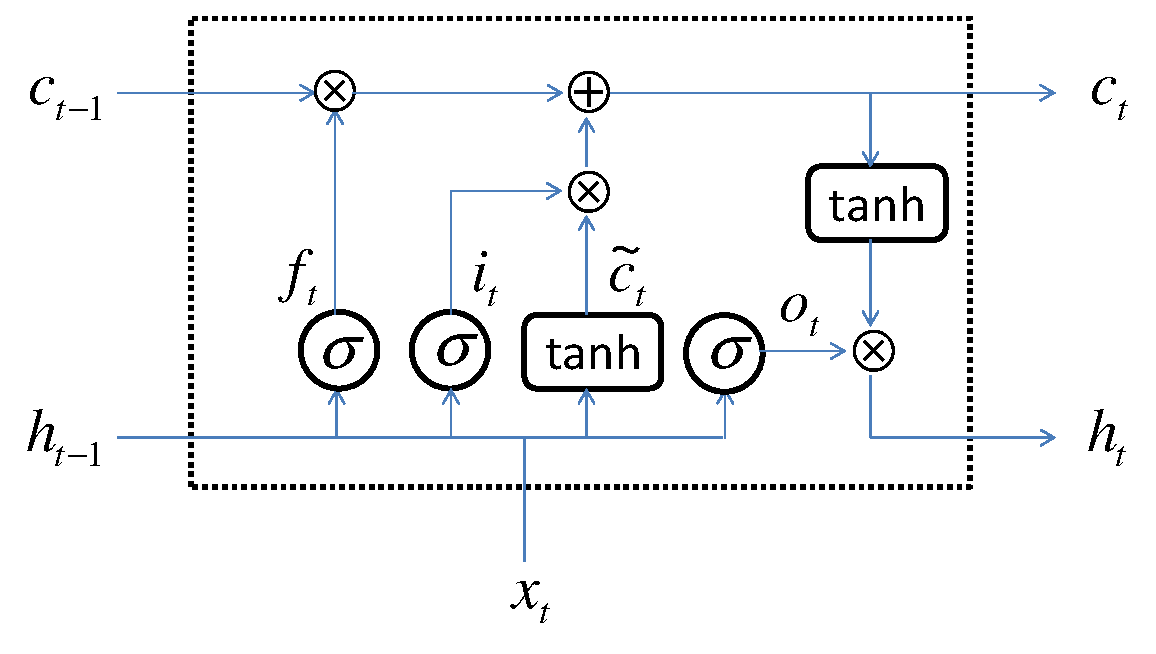
\includegraphics[width=80mm]{images/TsuruokaLab/lstm_yt.eps}
 \end{center}
 \caption{Long Short-Term Memory}
 \label{fig:lstm_yt}
\end{figure}

自然言語処理では,上述の問題点を解消し,高精度なリカレントニューラルネットワークを実現
する手法としてLSTM (Long Short-Term Memory) \cite{hochreiter1997long} や 
GRU (Gated Recurrent Unit) \cite{chung2014empirical} と呼ばれる
構造がよく用いられる.図\ref{fig:lstm_yt}に LSTM のユニットの構造を示す.
LSTM では,リカレントニューラルネットワークの通常の状態ベクトルで
ある $\boldsymbol{h}_{t}$ に加えて,メモリーセルと呼ばれる状態ベクトル $\boldsymbol{c}_{t}$ を持ち,
どのような情報をどのような場合に記憶(あるいは忘却)するかを細かく制御する「ゲート」と
呼ばれる機構を備えている.具体的には,LSTM の状態は,
\begin{eqnarray}
\boldsymbol{i}_t &=& \sigma(\boldsymbol{W}^{(i)} \boldsymbol{x}_t + \boldsymbol{U}^{(i)} \boldsymbol{h}_{t-1} + \boldsymbol{b}^{(i)})\\
\boldsymbol{f}_t &=& \sigma(\boldsymbol{W}^{(f)} \boldsymbol{x}_t + \boldsymbol{U}^{(f)} \boldsymbol{h}_{t-1} + \boldsymbol{b}^{(f)})\\
\boldsymbol{o}_t &=& \sigma(\boldsymbol{W}^{(o)} \boldsymbol{x}_t + \boldsymbol{U}^{(o)} \boldsymbol{h}_{t-1} + \boldsymbol{b}^{(o)})\\
\boldsymbol{\tilde{c}}_t &=& \sigma(\boldsymbol{W}^{(\tilde{c})} \boldsymbol{x}_t + \boldsymbol{U}^{(\tilde{c})} \boldsymbol{h}_{t-1} + \boldsymbol{b}^{(\tilde{c})})\\
\boldsymbol{c_t} &=& \boldsymbol{i}_t \odot \boldsymbol{\tilde{c}}_t + \boldsymbol{f}_t \odot \boldsymbol{c}_{t-1} \\
\boldsymbol{h_t} &=& \boldsymbol{o}_t \odot \tanh(\boldsymbol{c}_t)
\end{eqnarray}

\noindent
という式によって更新される.ただし,$\sigma(\cdot)$はシグモイド関数,$\odot$ はベクトルの要素積を表す.
$\boldsymbol{i}_t$,$\boldsymbol{f}_t$,$\boldsymbol{o}_t$ はそれぞれ,入力ゲート,忘却ゲート,出力ゲート
と呼ばれるベクトルであり,状態ベクトルの更新処理を制御する.

LSTM は,ニューラルネットワークを用いた自然言語処理で広く用いられており,いまでは多くの深層学習ライブラリで,
高性能なリカレントニューラルネットワークを実現する
標準的な「部品」として提供されている.本実験課題でも,LSTM を実験参加者が直接実装する必要はない.

%エンコーダーデコーダーモデルによる機械翻訳が成功したのはLSTMによるところが大きい.



\section{エンコーダ・デコーダモデル}

現在のニューラル機械翻訳技術のベースとなっているエンコーダ・デコーダモデル (encoder-decoder model) \cite{sutskever2014seq} 
では,2つのリカレントニューラルネットワークを使用する(図\ref{fig:encdec}).ひとつはエンコーダと呼ばれ,
翻訳元の文の単語を順次読み込み,文全体の内容を表す実数値ベクトルを生成する
役割を担う.もうひとつのリカレントニューラルネットワークはデコーダと呼ばれ,エンコーダ
が出力した実数値ベクトルを初期状態とし,上述の言語モデルと同様の仕組みで翻
訳先の単語列を出力する.
文全体の内容をひとつの実数値ベクトルで表現してしまおうというのはいかにも乱暴だが,
このような単純な仕組みで機械翻訳が実現できてしまうというのは驚きである.


\begin{figure}[t]
 \begin{center}
  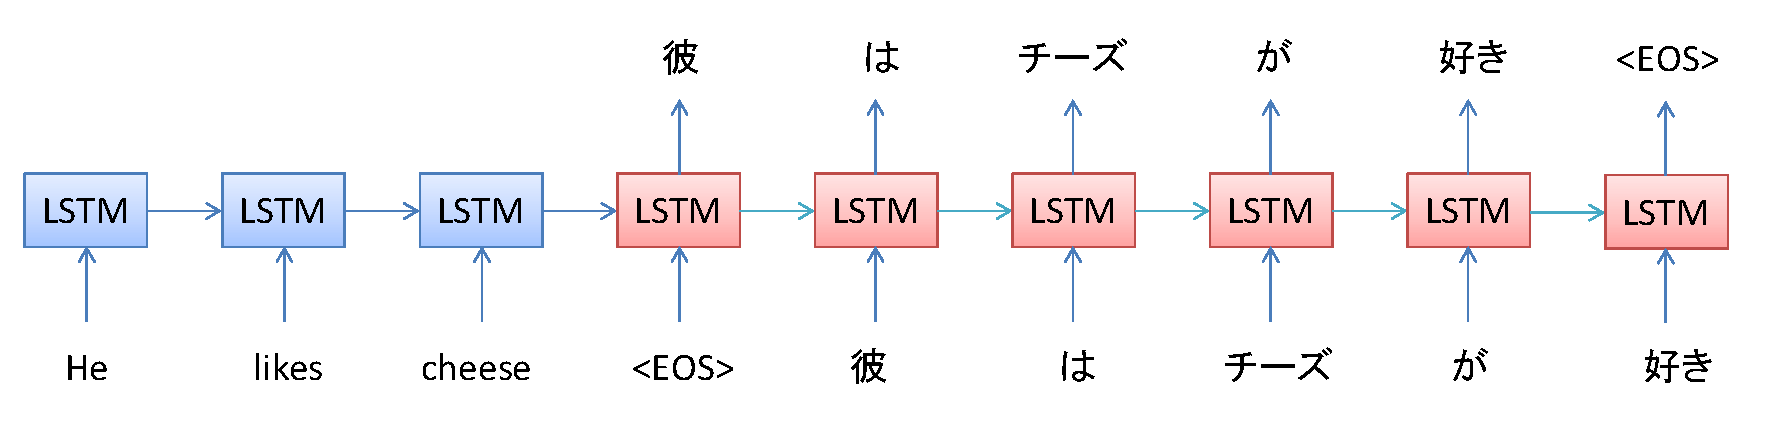
\includegraphics[width=140mm]{images/TsuruokaLab/encdec.eps}
 \end{center}
 \caption{エンコーダ・デコーダモデル}
 \label{fig:encdec}
\end{figure}

エンコーダ・デコーダモデルの学習は end-to-end で行う.つまり,エンコーダとデコーダを
それぞれ独立に学習されるのではなく,ひとつの大きなニューラルネットワークとして,
翻訳元の文から生成される翻訳先の単語列に関するモデルの対数尤度を最大化するようにパラメータ
を最適化する.


%\begin{equation}
%p(y_j | \boldsymbol{y}_{<j},\boldsymbol{x}) = \mbox{softmax}(\boldsymbol{W}_s s_j + b_s)
%\end{equation}

このような学習に必要なのは,「パラレルコーパス」と呼ばれる学習データである.
パラレルコーパスとは,文同士の
翻訳関係の対応がついている2言語のコーパスである.たとえば,機械翻訳モデル
の学習・評価用データとしてよく用いられるWMTデータセットでは,英仏では約3600
万文ペア,英独では約500万文ペアが提供されている.学習データの量が多ければ
多いほど翻訳精度が向上するというのは従来の統計的機械翻訳と同様だが,
ニューラル機械翻訳の場合は特にその傾向が強いと言われている.


\section{アテンション}

ニューラル機械翻訳のレベルを大きく引き上げたのは,アテンション(attention)と呼ばれ
る仕組みである \cite{bahdanau2015nmt}.これは,デコーダが各単語を出力する際の
情報として,エンコーダにおける各単語の隠れ状態の重み付き平均を入力として用いる
という方法で,翻訳元の文の文脈情報をより詳細にとらえることができるようになる.アテンションの
機構が導入されたことによってニューラル機械翻訳の精度は大きく向上し,従来の統計的機
械翻訳モデルの性能を凌駕することとなった.

\section{その他の応用}

Seq2seq モデルは,機械翻訳だけでなく様々な自然言語処理タスクに利用されている.
代表的な応用に,対話 \cite{vinyals2015neural},文書要約 \cite{rush2015neural},
質問応答 \cite{pmlr-v48-kumar16} などがある.

%\subsection{機械翻訳}



%\subsection{ニューラル会話モデル}



%\subsection{実験課題}


%https://github.com/chainer/chainer/tree/master/examples/seq2seq

